\documentclass[fleqn,final]{beamer}
\mode<presentation>
{
  \usetheme{ForumStatBlau}
}
\usepackage{times}
\usepackage{etex}
\usepackage{amsmath,amssymb}
%\usepackage{sfmath} % for sans serif math fonts; wget http://dtrx.de/od/tex/sfmath.sty
\usepackage[english]{babel}
\usepackage[ansinew]{inputenc}
\usepackage[orientation=portrait,size=a0,scale=1.25,debug]{beamerposter}
\usepackage{booktabs,array}
\usepackage{listings}
\usepackage{picins,graphicx}
\usepackage{xspace}
\usepackage{keyval}

\usepackage{wrapfig}
\usepackage{fp}
\usepackage{ifthen}
\usepackage[T1]{fontenc}
\usepackage{tikz,colortbl,pgf,pgfarrows,pgfnodes,pgfautomata,pgfheaps,pgfshade,eurosym, dsfont}

\usepackage{pgfplots}
%\pgfplotsset{compat=1.8}

\listfiles
\newcommand*{\signstream}{SignStream\texttrademark\xspace}
\newcommand{\WichtigFarbe}{\color{red}}%
\newcommand{\TextFarbe}{\color{black}}%


\def\bs{\boldsymbol}
\definecolor{darkblue}{rgb}{0.28,0,0.60}
\definecolor{hblue}{rgb}{0.70,0.7,1}
\definecolor{NR0}{rgb}{1,1,1}
\definecolor{NR1}{rgb}{1,1,0.8}
\definecolor{NR2}{rgb}{1,1,0.5}
\definecolor{NR3}{rgb}{1,1,0.25}
\definecolor{NR4}{rgb}{1,1,0.0}
\definecolor{NR5}{rgb}{1,0.75,0.0}
\definecolor{NR6}{rgb}{1,0.5,0.0}
\definecolor{NR7}{rgb}{1,0.25,0.0}
\definecolor{NR8}{rgb}{1,0,0.0}

\setbeamertemplate{navigation symbols}{}
\setbeamerfont{title}{series=\bfseries}

%\setbeamercolor{palette primary}{fg=yellow,bg=yellow} % changed this
%\setbeamercolor{palette secondary}{use=structure,fg=structure.fg!100!green} % changed this
%\setbeamercolor{palette tertiary}{use=structure,fg=structure.fg!100!green} % changed this
%\setbeamercolor{frametitle}{fg=UTblue}
\setbeamerfont{frametitle}{series=\bfseries}
\setbeamertemplate{frametitle}
{
\begin{centering}
\insertframetitle\vspace*{-4mm}\par
\end{centering}
}

\newcommand{\convD}{\stackrel{\text{d}}{\longrightarrow}}
\newcommand{\E}{\text{E}\,}
\newcommand{\var}{\text{V}\,}

% Display a grid to help align images
%\beamertemplategridbackground[1cm]
%\pgfdeclareimage[width=25cm]{CR}{graphs/CR}
\pgfdeclareimage[width=9.5cm]{RRMSE1}{RRMSE1}
\pgfdeclareimage[width=9.5cm]{RB1}{RB1}
\pgfdeclareimage[width=9.5cm]{RRMSEp1}{RRMSEp1}
\pgfdeclareimage[width=9.5cm]{RBp1}{RBp1}
\pgfdeclareimage[height=11cm]{histoposter1}{histoposter1}
\pgfdeclareimage[height=11cm]{histoposter2}{histoposter2}
\pgfdeclareimage[width=22cm]{Spatial}{Spatial}

\title{\huge Small Area Estimation of Poverty Indicators using Interval Censored Income Data} %konkreter Titel!!
\author{\large Paul Walter, Marcus Gro�, Timo Schmid \& Nikos Tzavidis}
\institute{Freie Universit�t Berlin \& University of Southampton} % (optional, but mostly needed)

\date{today}


\begin{document}

\begin{frame}{}
      
%%%%%%%%%%%%%%%%%%%%%%%%%%%%%%%%%%%%%%%%%%%%%%%%%%%%%%%%%%%%%%%%%%%%%%%%%%%%%%%%%
\vspace{-1cm} 
 \begin{columns}[t]
      \begin{column}{.50\linewidth}
        \begin{block}{\rule[-2.5mm]{0cm}{1cm}\textsc{1. Motivation}}


\begin{itemize}\small{
\item In order to fight poverty, it is essential to have knowledge about its spatial distribution.
\item Small area estimation (SAE) methods enable the estimation of poverty indicators at a geographical level where direct estimation is either not possible, due to a lack of sample size or very imprecise (Rao \& Molina , 2015).
\item One commonly used SAE method is the empirical best predictor (EBP) (Molina, 2010).
\item Estimation becomes imprecise, when due to confidentially or other reasons the dependent variable in the underlying mixed model, such as income, is censored to particular intervals.
\item To get more precise estimates, two methodologies, one based on the expectation maximization algorithm (EM) (Dempster et al., 1977) (Stewart, 1983) and one based on the stochastic expectation maximization (SEM) algorithm are introduced (Caleux, 1985).



}

\end{itemize}
\vspace{0.5cm}
\textcolor{blue}{How do the proposed methods assist in improving the precision of small area prediction when the dependent variable is censored to particular intervals?	} 		%		}
\vspace{0.5cm}

\end{block}
\vspace{-1cm}
%%%%%%%%%%%%%%%%%%%%%%%%%%%%%%%%%%
%%%%%%%%%%%%%%%%%%%%%%%%%%%%%%%%%%%%%%%%%%%%%%%%%%%%%%%%%%%%%%%%%%%%%%%%%%%%%%%%%%%%%%%%%%%%%%%%%%%%%%%%%%%%%%%
%%%%%%%%%%%%%%%%%%%%%%%%%%%%%%%%%%%%%%%%%%%%%%%%%%%%%%%%%%%%%%%%%%%%%%%%%%%%%%%%%	 	

\begin{block}{\rule[-2.5mm]{0cm}{1cm}\textsc{2. The EBP Approach (Molina \& Rao, 2010)}}
\begin{columns}[t]
\begin{column}{.53\linewidth}
{\small 
\vspace{-1.3cm}	
\begin{block}{\small{Nested error linear regression model (1) }}
\vspace{-1.3cm}	
\begin{align}\label{Mixed Model}
y_{ij}&=\mathbf{x}_{ij}^{T}\boldsymbol\beta + u_i + e_{ij}, \,\,\,\,\,\,j=1,\ldots,n_i,\,\,\,\,\,\,i=1,\ldots, D,\notag \\
u_i &\overset{iid}{\sim} N(0,\sigma^2_u), \text{the random area-specific effects}\\
e_{ij}& \overset{iid}{\sim}N(0,\sigma^2_e), \text{ the unit-level error terms}\notag
\end{align}
\textcolor{blue}{where $y_{ij}$ is unknown and only observed to fall into a certain interval \((A_{k-1},A_{k})\) on a continuous scale and \(k_{ij}\) \((1\leq k_{ij} \leq K)\) is the indicator into which of the intervals \(y_{ij}\) falls.}
\begin{itemize}
\item Use sample data to estimate $\beta$, $\sigma_u$, $\sigma_e$, $u_i$

\item Generate $u_i^*\sim~N(0,\hat\sigma_u^2)$ \& $e_{ij}^*\sim~N(0,\hat\sigma_e^2)$
\end{itemize}



\end{block}
}
\end{column}			

\begin{column}{.40\linewidth}
{\small 			
\vspace{-1.3cm}	
\begin{block}{\small{Arbitrary data example }}

\begin{table}[ht]
\begin{center}
\footnotesize
\begin{tabular}{ccccc}
\hline
ID & Unobserved $y_{ij}$ & Observed interval & $k_{ij}$ &$x_{ij}$\\
\hline
1 & 1251 & $[1000,1500)$ & 3 & 861\\
2 & 498 & $[0,500)$& 1 & 311 \\
3 & 898 & $[500,1000)$& 2 & 557 \\
4 & 753 & $[500,1000)$& 2 & 421\\
5 & 325 & $[0,500)$& 1 & 306\\
$\cdot$ &$\cdot$ & $\cdot$ & $\cdot$ \\
$\cdot$ &$\cdot$ & $\cdot$ & $\cdot$ \\
$\cdot$ &$\cdot$ & $\cdot$ & $\cdot$ \\
N & 5212 & $[4000,8000)$& 8 & 1350 \\
\hline
\end{tabular}
\end{center}
\end{table}

\end{block}



}
\end{column}
		  	 					
\end{columns}
\vspace{-0.7cm}	
{\small
{\color{blue}{Micro-simulating a synthetic population:}}
\begin{itemize}

\item Generate a synthetic population under the model a large number of times each time estimating the target parameter.

\item Linear and non-linear poverty indicators can be computed.

\end{itemize}
}
%%%%%%%%%%%%%%%%%%%%%%%%%%%%%%%%%%%%%%%%%%%%%%%%%%%%%%%%%%%%%%%%%%%%%%%%%%%%%%%%%
\end{block}	 	
%%%%%%%%%%%%%%%%%%%%%%%%%%%%%%%%%%%%%%%%%%%%%%%%%%%%%%%%%%%%%%%%%%%%%%%%%%%%%%%%%		



%%%%%%%%%%%%%%%%%%%%%%%%%%%%%%%%%%%%%
%%%%%%%%%%%%%%%%%%%%%%%%%%%%%%%%%%%%%%%%%%%%%%%%%%%%%%%%%%%%%%%%%%%%%%%%%%%%%%%%%%%%%%%%%%%%%%%%%%%%%%%%%%%%%%%%%%
\vspace{-1.2cm}
        
%%%%%%%%%%%%%%%%%%%%%%%%%%%%%%%%%%%%%%%%%%%%%%%%%%%%%%%%%%%%%%%%%%%%%%%%%%%%%%%%%

\begin{block}{\rule[-2.5mm]{0cm}{1cm}\textsc{3. Methodology}}

\begin{itemize}
\small{
\item Reconstructing the distribution of the unknown \(y_{ij}\) is necessary to estimate the parameters of model (1).
\item From Bayes theorem it follows that \(f(y_{ij}|x_{ij}, k_{ij})\propto f(k_{ij}|y_{ij},x_{ij})f(y_{ij}|x_{ij})\) with

\begin{columns}[t]
\begin{column}{.4\linewidth}
\vspace{-1.0cm}
\begin{equation*}
f(k_{ij}|y_{ij},x_{ij})=\begin{cases}
  1,  & \text{if } A_{k-1} \leq y_{ij} \leq A_{k} \\ 
  0, & \text{else } 
\end{cases}
\end{equation*}
\end{column}
\begin{column}{.4\linewidth}

and \( f(y_{ij}|x_{ij})  \sim \enspace N(x_{ij}^{T}\beta+u_{i}, \sigma^{2}_{e}).\)
\end{column}
\end{columns}

}
\end{itemize} 
 
\end{block}

%%%%%%%%%%%%%%%%%%%%%%%%%%%%%%%%%%%%%%%%%%%%%%%%%%%%%%%%%%%%%%%%%%%%%%%%%%%%%%%%%%%%%%%%%%%%%%%%%%%%%%%%%%%%%%%%%%
\vspace{-1.2cm}
        
%%%%%%%%%%%%%%%%%%%%%%%%%%%%%%%%%%%%%%%%%%%%%%%%%%%%%%%%%%%%%%%%%%%%%%%%%%%%%%%%%

\begin{block}{\rule[-2.5mm]{0cm}{1cm}\textsc{4. Estimation and Computational Details (EM and SEM Algorithm)}}


\begin{enumerate}
\small{
\item Estimate \(\hat{\theta}=(\hat{\beta} \), \(\hat{u_{i}} ,\hat{\sigma}^{2}_{e})\) from model (1) using the midpoints of the intervals as a substitute for the unknown \(y_{ij}\). 

\item Generate pseudo samples to reconstruct the distribution of the unknown \(y_{ij}\):
\begin{itemize}


\item \textbf{EM:} Estimate \(E[I(A_{k-1} \leq y_{ij} \leq A_{k}) \times \pi(y_{ij}|x_{ij})]\), the expected value of a two sided truncated normal distributed variable as pseudo \(\tilde{y}_{ij}\): 
\begin{equation*}
\tilde{y}_{ij}=E[I(A_{k-1} \leq y_{ij} \leq A_{k}) \times \pi(y_{ij}|x_{ij})]=(x_{ij}^{T}\hat{\beta}+\hat{u}_{j})+\hat{\sigma}_{e}\frac{\phi(Z_{k-1})-\phi(Z_{k})}{\Phi(Z_{k})-\Phi(Z_{k-1})},
\end{equation*}
obtaining \((\tilde{y}_{ij}, x_{ij})\) for \(j=1, \ldots n_{i}\) and \(i=1,\ldots, D\). The conditional variance is given by the variance of a two sided truncated normal distributed variable as
\begin{equation*}
Var(y_{ij}|x_{ij}, k_{ij}, u_{i})=\hat{\sigma}_{e}^{2}\underbrace{\left\{\left[\frac{Z_{k-1}\phi(Z_{k-1})-Z_{k}\phi(Z_{k})}{\Phi(Z_{k})-\Phi(Z_{k-1})}\right]-\left[\frac{\phi(Z_{k-1})-\phi(Z_{k-1})}{\Phi(Z_{k})-\Phi(Z_{k-1})}\right]^2\right\}}_{:=s_{ij}}
\end{equation*}
with \(Z_{k}=(A_{k}-(x_{ij}^{T}\hat{\beta}+\hat{u}_{i}))/\hat{\sigma}_{e}\). 

\item \textbf{SEM:} Sample from the conditional distribution \(\pi(y_{ij}|x_{ij})\) by drawing  randomly  from  \(N(x_{ij}^{T}\hat{\beta}+\hat{u}_{i}, \hat{\sigma}^{2}_{e}) \) within the given interval \(A_{k-1} \leq y_{ij} \leq ,A_{k}\) obtaining \((\tilde{y}_{ij}, x_{ij})\) for \(j=1, \ldots n_{i}\) and \(i=1,\ldots, D\).
\end{itemize}
\item Re-estimate the vector \(\hat{\theta} \) from model (1) by using the pseudo sample \((\tilde{y}_{ij}, x_{ij})\) obtained in step 2. The variance \(\hat{\sigma}_{e}^{2}\) is given by:


\begin{itemize}
\begin{columns}[t]
\begin{column}{.4\linewidth}

\item \textbf{EM}:  \begin{equation*}
\hat{\sigma}_{e}^2=\frac{\sum_{j=1}^{n_{i}}\sum_{i=1}^{D}(\tilde{y}_{ij}-(x_{ij}^{T}\hat{\beta}+\hat{u}_{i}))^2}{\sum_{j=1}^{n_{i}}\sum_{i=1}^{D}(1-s_{ij})}
\end{equation*}
\end{column}
\begin{column}{.4\linewidth}
\item \textbf{SEM}:
\begin{equation*}
\hat{\sigma}_{e}^2=\frac{\sum_{j=1}^{n_{i}}\sum_{i=1}^{D}(\tilde{y_{ij}}-(x_{ij}^{T}\hat{\beta}+\hat{u}_{i}))^2}{(N-1)}
\end{equation*} 

\end{column}
\end{columns}
\end{itemize}


\item Number of iterations:
\begin{itemize}


\item \textbf{EM:} Iterate steps 2.-3. until convergence.
\item \textbf{SEM:} Iterate steps 2.-3. \(B+M\) times, with \(B\) burn-in iterations and \(M\)  additional iterations. 
\end{itemize}

\item Final parameter estimation:

\begin{itemize}

\item \textbf{EM:} Obtain \(\hat{\theta} \) from the last iteration step. 
\item \textbf{SEM:} Discard the burn-in iterations and estimate \(\hat{\theta} \) by averaging the obtained \(M\) estimates.

\end{itemize}
}
\end{enumerate}
\end{block}




%%%%%%%%%%%%%%%%%%%%%%%%%%%%%%%%%%%%%%%%%%%%%%%%%%%%%%%%%%%%%%%%%%%%%%%%%%%%%%%%%%%%%%%%%%%%%%%%%%%%%%%%%%%%%%%%%%%%%%%%%%%%%%%%



  \end{column}
%%%%%%%%%%%%%%%%%%%%%%%%%%%%%%%%%%%%%%%%%%%%%%%%%%%%%%%%%%%%%%%%%%%%%%%%%%%%%%%%%
%%%%%%%%%%%%%%%%%%%%%%%%%%%%%%%%%%%%%%%%%%%%%%%%%%%%%%%%%%%%%%%%%%%%%%%%%%%%%%%%%
%%%%%%%%%%%%%%%%%%%%%%%%%%%%%%%%%%%%%%%%%%%%%%%%%%%%%%%%%%%%%%%%%%%%%%%%%%%%%%%%%
%%%%%%%%%%%%%%%%%%%%%%%%%%%%%%%%%%%%%%%%%%%%%%%%%%%%%%%%%%%%%%%%%%%%%%%%%%%%%%%%%
%%%%%%%%%%%%%%%%%%%%%%%%%%%%%%%%%%%%%%%%%%%%%%%%%%%%%%%%%%%%%%%%%%%%%%%%%%%%%%%%%

    \begin{column}{.46\linewidth}
  
  %%%%%%%%%%%%%%%%%%%%%%%%%%%%%%%%%%%%%%%%%%%%%%%%%%%%%%%%%%%%%%%%%%%%%%%%%%%%%%%%%%%%%%%%%%%%%%%%%%%%%%%%%%%%%%%%%%%%%%%%%%%%%%%%%%%%%%%%%%
\begin{block}{\rule[-2.5mm]{0cm}{1cm}\textsc{4. Simulation setup}}

\begin{itemize}\small{
\item
Assume a finite population $U$ of size $N =40000$, partitioned into $D=40$ regions $U_1,U_2,\ldots,U_D$ of sizes $N_i=1000$
\item
Let $n_i$ be the sample size in region $i$ with $n_i=20$ and $\sum_{i=1}^{D}n_i=800$
\item 500 samples were randomly drawn from the following scenario:
}
\end{itemize}  

\vspace{-1.2cm}
{\small
\begin{align*}
y_{ij}&=1300 - 1x_{ij} + u_i + e_{ij},\,\,\,\,\,\,  x_{ij} \sim GB2(5.0,800,0.4,0.5), \\
u_i &\overset{iid}{\sim} N(0,1\times 10^4),\,\,\,\,\,\, e_{ij} \overset{iid}{\sim}N(0,1.5\times 10^5),\,\,\,\,\,\, j=1,\ldots,n_i, \,\,\,\,\,\,i=1,\ldots,D.
\end{align*}
}
\vspace{-1.5cm}
\begin{table}[ht]
\begin{center}
\tiny
\begin{tabular}{lccccccccc}
\hline
\multicolumn{10}{c}{\textbf{Interval censoring of $Y_{ij}$}}\\
\hline
Intervals scenario 1 & $[0,500)$& $[500,1000)$ & $[1000,1500)$ &$[1500,2000)$& $[2000,2500)$ & $[2500,3000)$ &$[3000,4000)$  & $[4000,8000)$ & $[8000,Inf)$\\ 
Frequencies scenario 1 & 34       & 705           & 4715         & 11908& 11975         & 6191         & 3300       & 1050 &122\\ 
\hline
Intervals scenario 2 &$[0,2000)$& $[2000,4000)$ & $[4000,6000)$ &$[6000,8000)$& $[8000,Inf)$ & & &&\\ 
Frequencies scenario 2 &17362       & 21466           & 893         & 157& 122         &       & & & \\ 
\end{tabular}
\end{center}
\end{table}
                        
\vspace{-0.5cm}                                            

        \end{block}
    
%%%%%%%%%%%%%%%%%%%%%%%%%%%%%%%%%%%%%%%%%%%%%%%%%%%%%%%%%%%%%%%%%%%%%%%%%
	\begin{block}{\rule[-2.5mm]{0cm}{1cm}\textsc{5. Simulation Results}}
	{\small
\textcolor{blue}{The following methods were applied for parameter estimation of model (1):}
\begin{itemize}
\item LME - Estimate the model parameters with the true \(y_{ij}\) to evaluate the performance of the estimation methods relying on the interval censored \(y_{ij}\).
\item MIDREG - Estimation based on the interval midpoints as proxy for the unknown \(y_{ij}\).
\item EM - Estimation based on the generated pseudo \(\tilde{y}_{ij}\). 
\item SEM - Estimation based on the drawn pseudo \(\tilde{y}_{ij}\), with 100, 200 and 400 iterations (SEM1, SEM2 and SEM3).
\item GRSST - Direct estimation using the GRSST estimator with \(B=5\) and \(M=20\) (Gro� et al. 2016). 
\end{itemize}	
	}
	
	\vspace{-1.3cm}
	\begin{column}{.98\linewidth}
	   \begin{block}{\small{Performance of the EBPs}}
	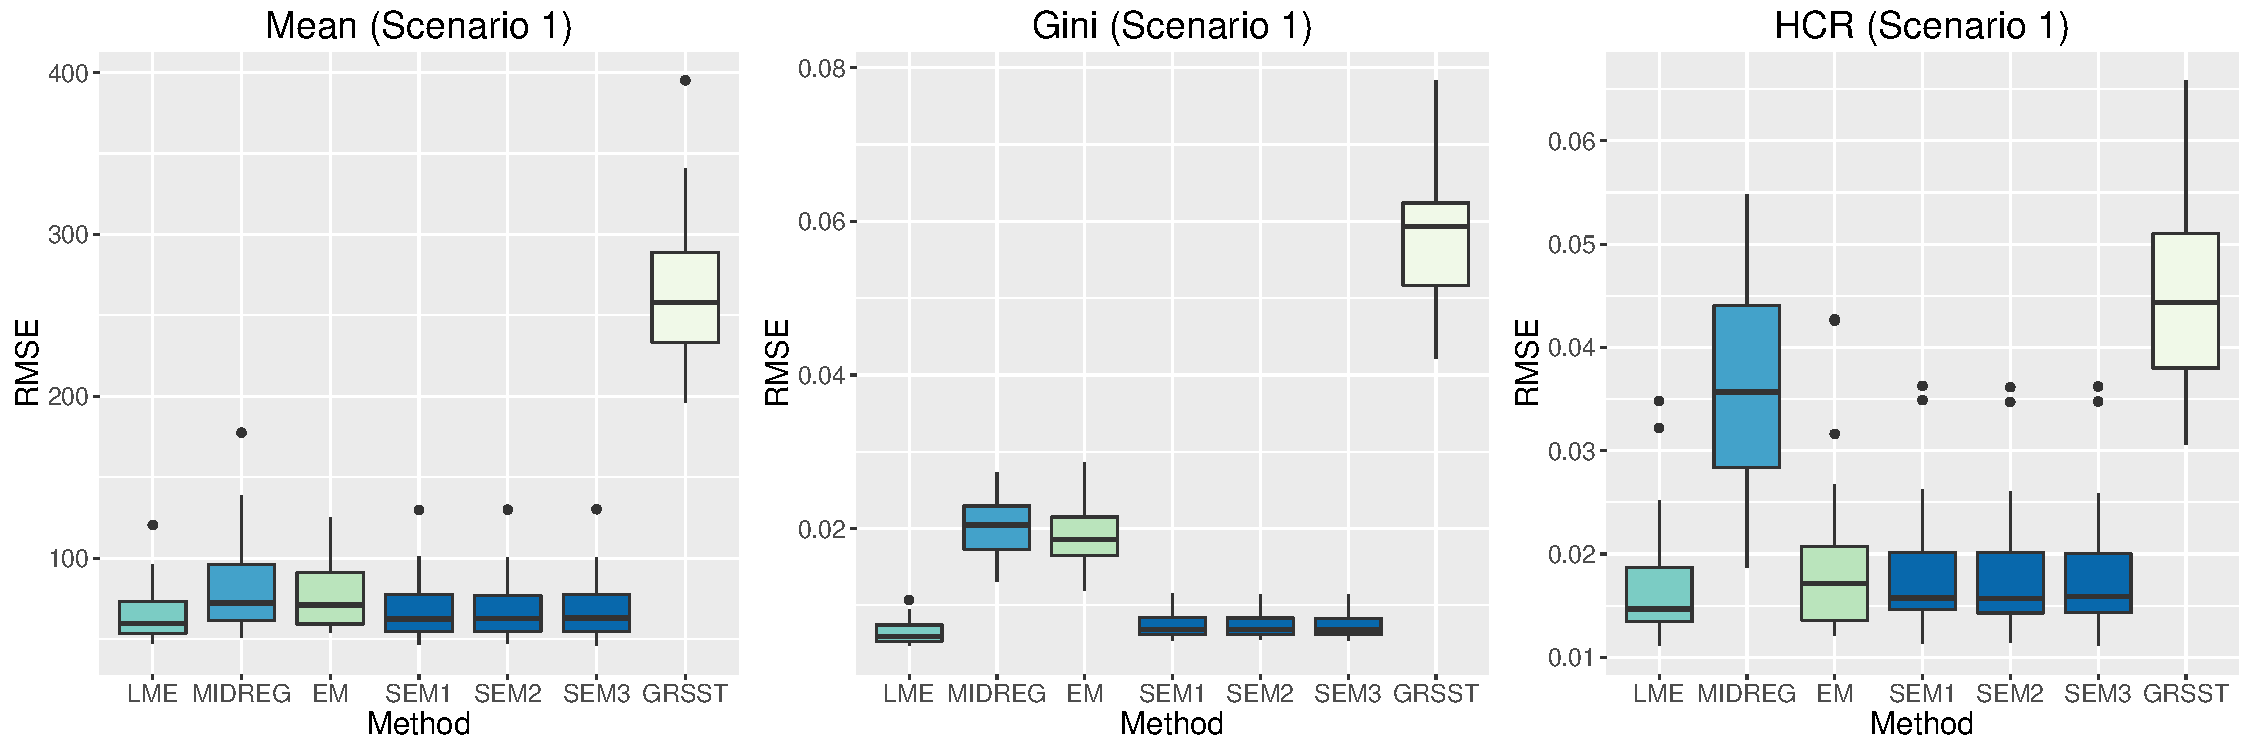
\includegraphics[height=12cm]{multibox_scenario1.pdf} \\
	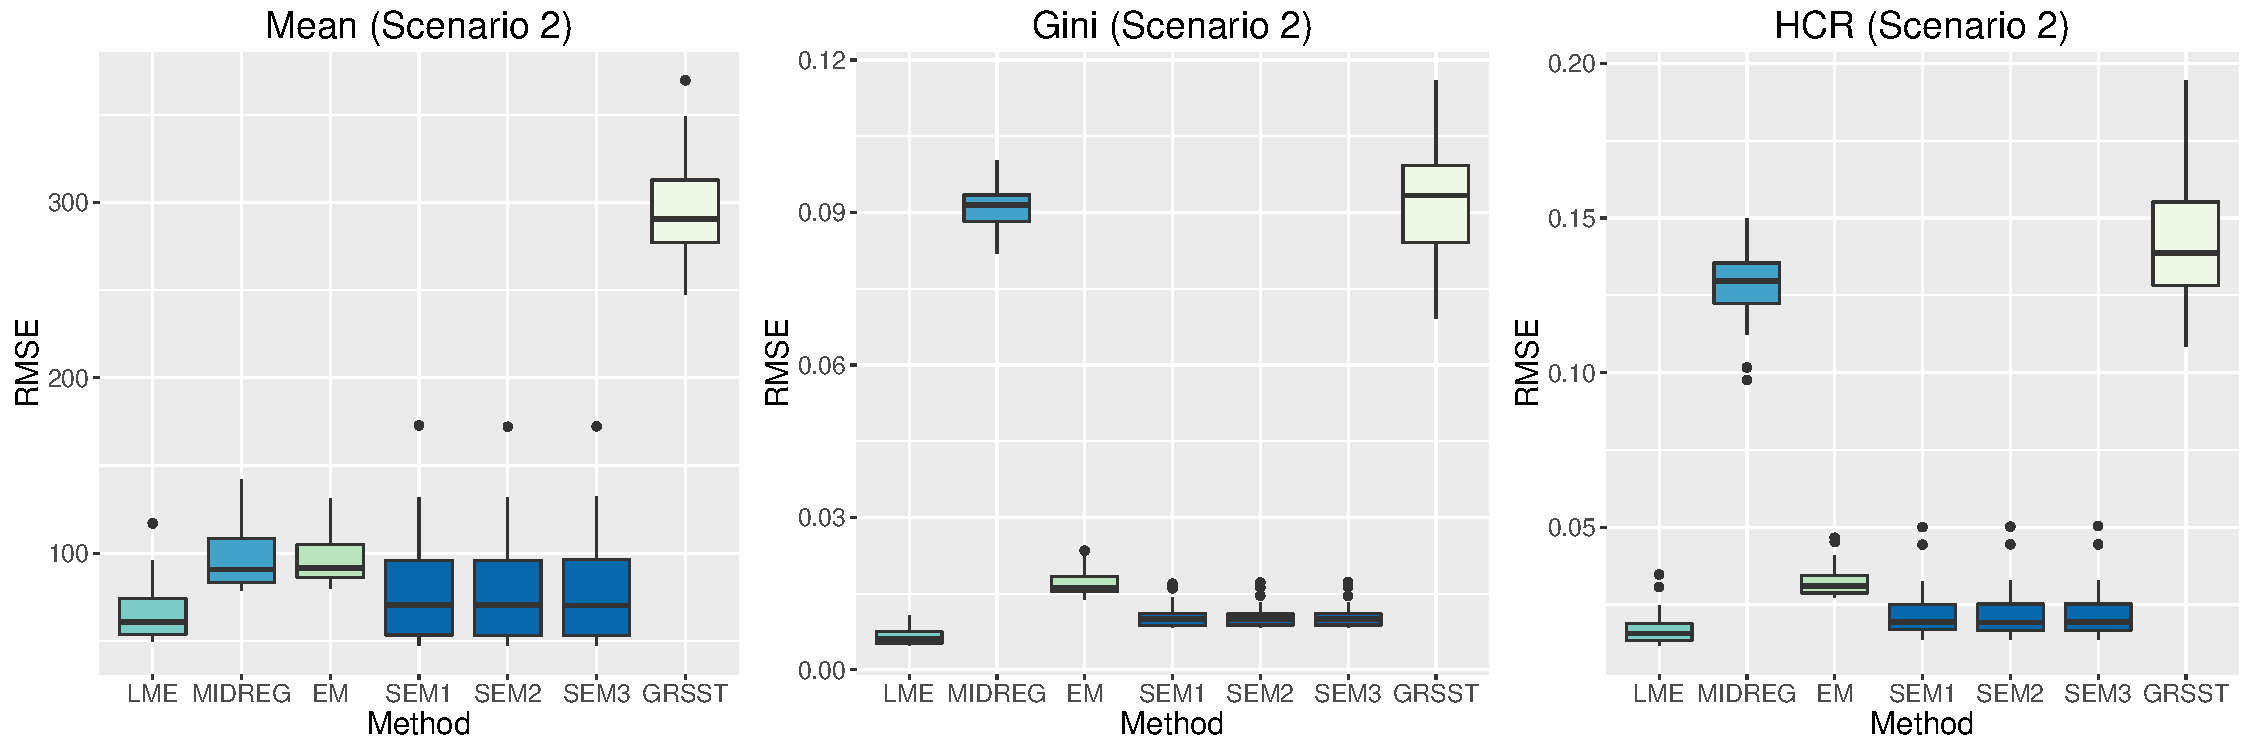
\includegraphics[height=12cm]{multibox_scenario2.pdf}
		
\end{block}
\end{column}
\vspace{-1.3cm}
	\begin{column}{.98\linewidth}
	   \begin{block}{\small{Density plots of $\hat{y}$ from a particular simulation run}}
	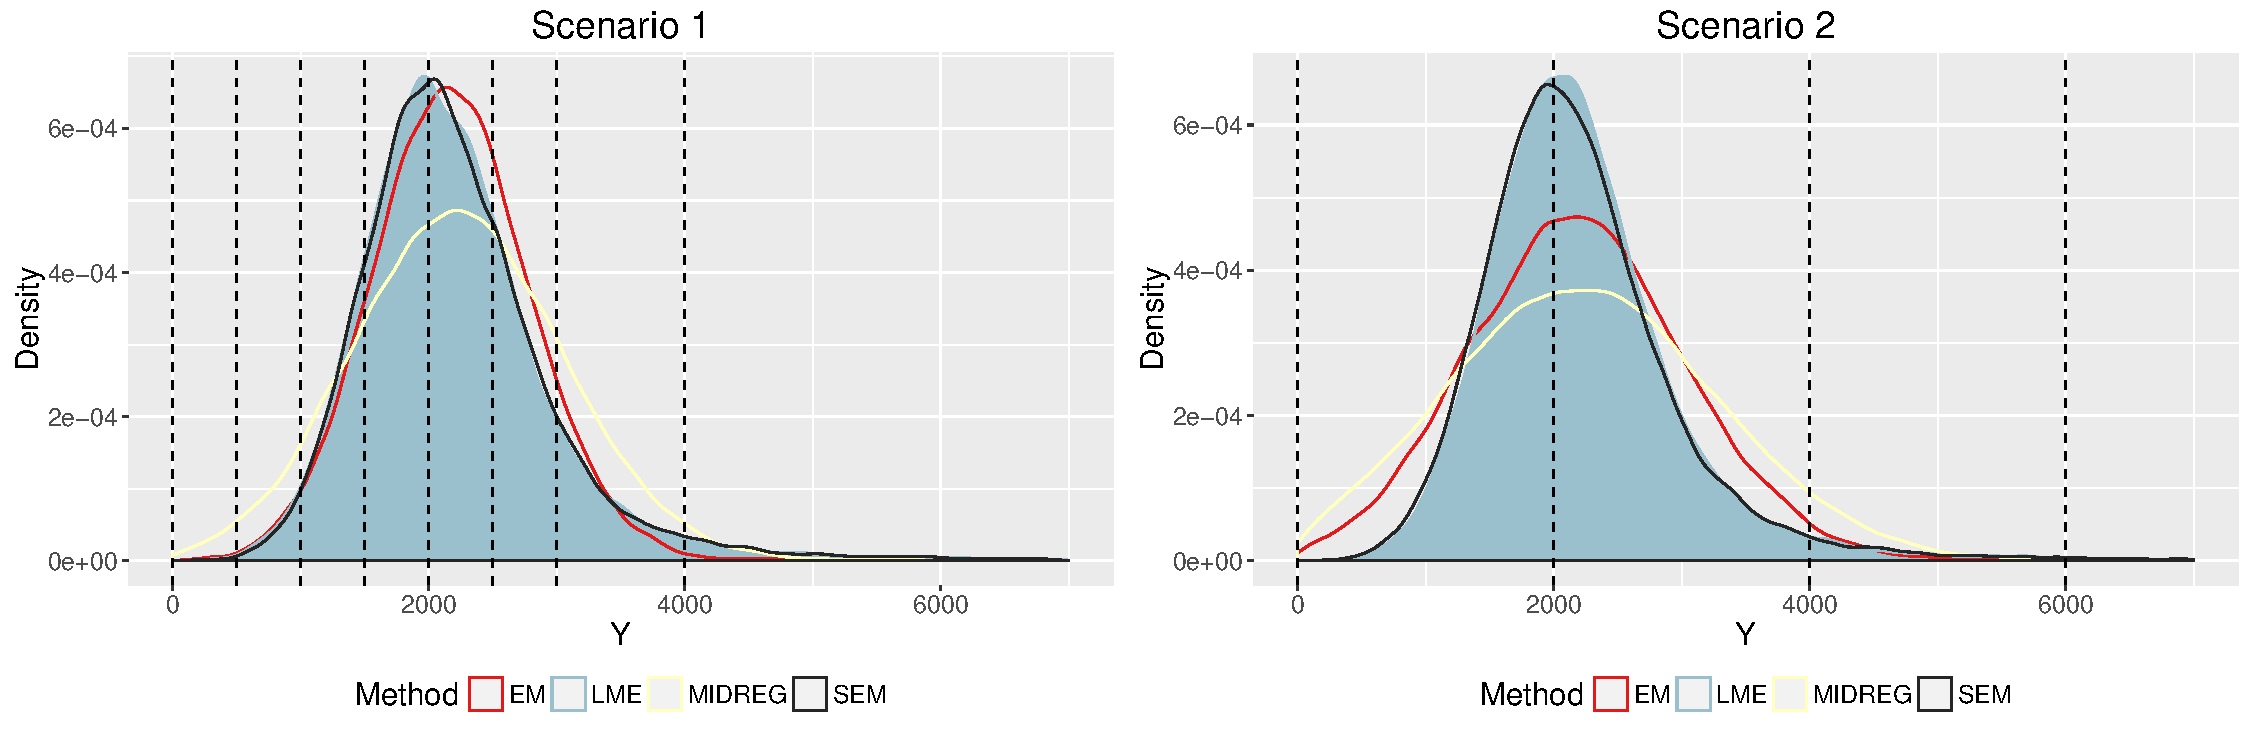
\includegraphics[height=12cm]{multidensity_EBP.pdf} 

		
\end{block}
\end{column}
\end{block}	 	
\vspace{-1cm}






%%%%%%%%%%%%%%%%%%%%%%%%%%%%%%%%%%%%%%%%%%%%%%%%%%%%%%%%%%%%%%%%%%%%%%%%%%%%%%%%%%%%%%%%%%%%%%%%%%%%%%%%%%%%%%%%%%%%%%%%%%%%%%%%%%%%%%%%%%

	 	
\begin{block}{\rule[-2.5mm]{0cm}{1cm}\textsc{6. Discussion and Outlook}}



\begin{itemize}
\item \textcolor{blue}{Simulation results show that the use of the SEM algorithm increases the accuracy, in terms of RMSE, in the EBPs.}
\item The amount of accuracy gained depends strongly on the number of intervals. However, the SEM algorithm still outperforms the other methods in the presence of many intervals.
\item A high number of iterations (e.g. 200 or 400) does not improve the precision any further.

\item \textbf{Further research:} How can possible violations of model assumptions be detected? How can transformations be applied for handling non-normally distributed error terms?  
\end{itemize}





		\end{block}	 	
%%%%%%%%%%%%%%%%%%%%%%%%%%%%%%%%%%%%%%%%%%%%%%%%%%%%%%%%%%%%%%%%%%%%%%%%%%%%%%%%%		
			
 \end{column}
\end{columns}



\vspace{-1cm}
   \begin{block}{References}
   \vspace{-0.3cm}

{\footnotesize

\noindent [1]  Rao, J.N.K. \& Molina, I. (2015),
 Small area estimation. John Wiley \& Sons.\\

\noindent [2] Foster, J., Greer, J. \& Thorbecke, E. (1984),
A class of decomposable poverty measures. Econometrica, 52(3):761-766.\\

\noindent [3] Molina, I. \& Rao, J.N.K. (2010),
Small area estimation of poverty indicators. 
Canadian Journal of Statistics, 38(3), 369-385.\\

\noindent [4] Caleux, G. \& Dieboldt, J. (1985),
The sem algorithm: a probalistic teacher algorithm derived
from the em algorithm for the mixture problem. 
Computational Statistics Quarterly, 2:73-82.\\

\noindent [5] Stewart, M. B. (1983),
On least square estimation when the dependent variable is grouped. 
Review of Economic Studies, 50(4):737-753.\\

\noindent [6] Dempster, A., Laird, N., \& Rubin, D. (1977),
Maximum likelihood from incomplete data via the em algorithm. 
Journal of the Royal Statistical Society. Series B (Methodological),
39(1):1 - 38.\\

\noindent [7] Gro�, M., Rendtel, U., Schmid, T., Schmon, S.\& Tzavidis, N. (2016),
Estimating the density of ethnic minorities and aged people in Berlin: multivariate kernel density estimation applied to sensitive georeferenced administrative data protected via measurement error.
Journal of the Royal Statistical Society. Series A.
\\


}


    \end{block}

\end{frame}


\end{document}

